%!TEX root = ../dissertation.tex
\begin{savequote}[60mm]
There is no scientific study more vital to man than the study of his own brain. Our entire view of the universe depends on it.\qauthor{Francis Crick}
\end{savequote}

% If the human brain were so simple that we could understand it, we would be so simple that we couldn’t.
% – Emerson M. Pugh

% The human brain, then, is the most complicated organization of matter that we know.     
% Isaac Asimov

% One of the difficulties in understanding the brain is that it is like nothing so much as a lump of porridge.
% Richard L. Gregory

% The brain is a monstrous, beautiful mess. Its billions of nerve cells - called neurons - lie in a tangled web that displays cognitive powers far exceeding any of the silicon machines we have built to mimic it.
% William Allman

\chapter{microRNA Dynamics in Cholinergic Differentiation of Human Neuronal Cells}

\newthought{Even though much has been achieved} in the integrative study of \ac{mir} control of gene expression, computational analysis of transcriptional interactions has not yet reached the level of sophistication needed for the accurate prediction of events inside mammalian cells. For this reason, combination of a bioinformatical assay with modern molecular biology methods can strengthen the message and reproducibility of any approach. The spectrum of processes worthy of study is as wide as modern biomedicine. Similarly, experimental models can span the entire repertoire available to a modern laboratory. The selection of a model adequate to the research question therefore is as important as diligent analysis and careful interpretation of results.

This chapter will discuss the current state of knowledge on brain transciptomics generally and in the specific case of cholinergic neurons in the \ac{cns}, and then go on to explain the steps I undertook to elucidate relevance of small RNA processes in central cholinergic systems. First, my aim was to clarify co-expression patterns of central cholinergic neurons, which required analysis of transcriptome data in single-cell resolution. Based on this information, I selected two human models of cholinergic neuronal differentiation and established a differentiation protocol amenable to RNA extraction and successive molecular biology assays, most importantly, \ac{seq}. The expression patterns so obtained were then used as basis of bioinformatics analyses using the database introduced in Chapter \ref{mirnet}, \textit{miRNet}. 

\section{Neuronal Transcriptomes - Background}
The mammalian brain requires a constant supply of oxygen and nutrients, because it does not provide storage for either. Though it only makes up approximately 2\% of the entire human body mass, its energy expenditure is around 20\% of the whole\cite{Raichle2002}. For this reason, there is no cubic micrometre of brain tissue (except for the ventricles) that is not infiltrated by multiple capillaries. Since the blood-brain-barrier is essentially provided by supporting glia cells surrounding all capillaries from the »inside« (see Fig. \ref{fig:bbb}, adapted from my second publication\cite{Lobentanzer2019b}), neurons constitute only a minority of brain tissues.

\begin{figure}
\includegraphics[width=\textwidth]{figures/bbb}
\caption[Short figure name.]{This is a figure that floats inline and here is its caption.
\label{fig:bbb}}
\end{figure}

Before the advent of single-cell \ac{seq}, studies that endeavoured to clarify the transcriptional profiles of neurons used microarray technology, which was only recently succeeded by \ac{seq} (also known as deep sequencing or next generation sequencing). For these methods, several cubic millimetres of brain tissue are required at the least; often, cubic centimetres are used. Thus, the resolution of the method and the actual cellular resolution differ by a factor of approximately \num{10000}. Additionally, even among the neuronal population, there is considerable heterogeneity and transcriptomic plurality; single brain regions rarely consist of less than 30 different neuron types, tightly packed next to each other, each with their own transcriptional identity\cite{Darmanis2015, Zeisel2015, Tasic2016, Habib2016, Zeisel2018}. These circumstances hold true for any mammal, and most of our knowledge stems from the analysis of our favourite research animal, the mouse. In humans, the complexity is only exacerbated; in fact, the elevation in \ac{cns} transcriptional complexity might be the reason for our superior cognitive abilities(cite).

Cholinergic neurons always constitute a minority in any neuronal population, sometimes to extremes. Most tissues are dominated by few neuron types, such as pyramidal cells in the cortex; the most common neurotransmitter types are GABAergic (inhibitory) and glutamatergic (excitatory), each with several subtypes. It is estimated that more than 80\% of cortical neurons are excitatory, and more than 90\% of synapses release glutamate\cite{Raichle2002}. The striatum is fairly well-populated with rather large cholinergic interneurons, and the basal forebrain holds a large amount of (smaller) cholinergic projection neurons (compare Fig. \ref{fig:projections}). However, in transcriptomic analyses, these tissues are seldom used, for lack of scientific interest, or because they are notoriously hard to access (the basal forebrain is small and deeply imbedded in the midbrain). The cortex, particularly the neocortex, is most often the tissue of choice in these studies, due to its scientific interest and accessibility. Though it contains only a minuscule amount of cholinergic interneurons whose identity still is a matter of debate, several of the recent single-cell \ac{seq} approaches have independently identified cholinergic interneurons in cortical regions (see Fig. \ref{fig:singlecell}). 

All of the above taken into consideration, several limitations apply when it comes to the selection of a cellular model for the cholinergic processes I aim to understand. A multicellular model is prohibited by the novelty of the subject; possibilities include \textit{in vivo} or \textit{ex vivo} experimentation on rodents or human (3D-)cell culture with multiple cell types. While the former certainly is closest to reality, the diseases of interest display a noticeable lack of transferability from lower mammals to human(cite). The latter, on the other hand, introduces a complexity not well suited to the level of knowledge we possess about the studied processes; in addition, these models are very new, and thus, too many variables would be unknown. For these reasons, I selected two mono-cultures of human neuronal cells for my experiments. I chose to introduce a second cellular model during the experimental phase, because some of the studied diseases display a clear sexual dimorphism; the first experiments were performed on the female-originated LA-N-2 cell line, and later, to explore sex-related differences, the male-originated LA-N-5 cells were added.

\section{Cortical Single-Cell RNA Sequencing}
To estimate the potential impact of the transcriptomes studied in our model on the diseases of interest, co-expression of the relevant genes has to be asserted. Similarly, if neurokines are to possess any relevance for cholinergic properties of central nervous cells, the cells in question would have to express molecular machinery required to receive neurokine signals. The advent of single-cell \ac{seq} for the first time enables the resolution of gene expression on a cellular basis, and thus the disentangling of spatially close individual neuron types (and other, non-neuronal \ac{cns} cells); most of this information would be lost by \ac{seq} performed on brain homogenate, even of a small biopsy. Differences in genes would be reduced to the universally expressed »housekeeping« genes, and in \acp{mir}, the situation would be worse, in parallel to their even more tissue-specific expression.

For this reason, I analysed all publicly available single-cell \ac{seq} datasets relevant to our questions, which provide a detailed tally of transcriptional subtypes in the \ac{cns}. More specifically, all studies that were available at the time focused on some subsection of the cortex (visual or somatosensory) or the hippocampus. Additionally, the data provided by those studies was in some cases pre-aggregated to represent groups of single neurons with similar transcriptomes\cite{Zeisel2015, Tasic2016}, in other cases, every single neuron was represented\cite{Darmanis2015, Habib2016}. 

An important quality-related parameter of a single-cell \ac{seq} experiment is the sequencing depth achieved per individual sequenced cell. Some datasets I screened do not provide sufficient depth to resolve genes with medium expression, which includes our primary cholinergic markers \textit{\ac{chat}} and \textit{\ac{slc}}. The datasets with adequate sequencing depth were filtered for their expression of these markers, and additionally characterised by their expression of common markers for cell types to be expected in the \ac{cns}. This resulted in a collection of transcriptomes for potentially cholinergic cells in the sampled brain regions, and allowed an assessment of their functional type and gene co-expression patterns in central cholinergic cells (Fig. \ref{fig:singlecell}).

\begin{figure}
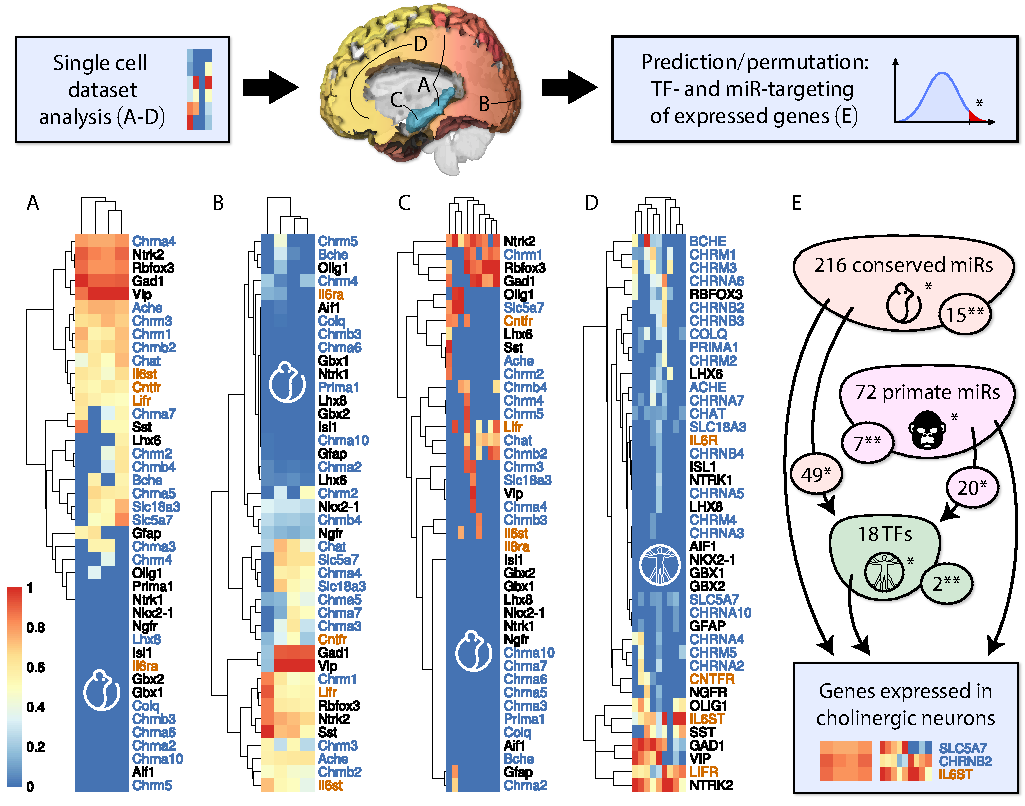
\includegraphics[width=\textwidth]{figures/singlecell}
\caption[Short figure name.]{This is a figure that floats inline and here is its caption.
\label{fig:singlecell}}
\end{figure}

Most cells identified as cholinergic by this definition expressed the general neuronal marker \textit{\acs{rbf}}, also known by its trivial name NeuN, but not the microglial marker \textit{\acs{aif}}. Few cells (or clusters of cells) expressed non-neuronal markers such as \textit{\acs{gfap}} (astrocytes) or \textit{\acs{oli}} (oligodendrocytes), hinting at sparse non-neuronal cholinergic functions. Cholinergic cells or clusters identified by the authors of the respective studies were classified as interneurons and co-expressed a number of known phenotypic neuronal markers, such as \textit{\ac{sst}} and \textit{\ac{vip}}.

Identified cholinergic cells also revealed a constant co-expression with neurokine-related genes, particularly the transmembrane neurokine receptors \ac{lifr} and \ac{ilst}, demonstrating a capacity to receive and process neurokine signals. In contrast, the high affinity receptor for \ac{ngf}, \textit{NTRK1}, is not expressed by many of the cholinergic neurons, fundamentally distinguishing these cells from the basal forebrain cholinergic projection neurons.
\todo{Clusters?}

\section{The Cellular Model}
A prominent example of human neuronal cell culture used in the identification and elucidation of cholinergic processes is the immortalised neuroblastoma cell line SH-SY5Y\cite{Biedler1978}. Derived from its parent line SK-N-SH, an adrenergic neuroblastoma\cite{Biedler1973}, it expressed ample amounts of \textit{\ac{ache}}, and thus had become a work horse in many cholinergic fields, such as Alzheimer's Disease (which is treated with \ac{ache} antagonists), pesticide development, and warfare(cite). However, in spite of its usefulness for processes involving \textit{\ac{ache}}, it turned out a less than optimal choice for the study of molecular events surrounding \textit{\ac{chat}} and \textit{\ac{slc}}, as it barely expresses both genes(cite), and cannot be coerced to elevate \textit{\ac{chat}} expression by the usual differentiation techniques (own experimentation, data not shown). Thus, for the questions asked in due course of this dissertation, SH-SY5Y does not qualify as adequate representation of a »cholinergic neuron«.

Following the elimination of SH-SY5Y as a suitable subject, I scoured the literature for candidates representing a cholinergic neuronal transcriptome, and found, among others, representatives of the LA-N neuroblastoma cell lines developed by R.C. Seeger around 1980\cite{Seeger1977, Seeger1982}. Neuroblastoma is a form of neuronal cancer often affecting small children, and, consequentially, the two cell lines used in my experiments are immortalised biopsies of a 3 year old girl (\acs{la2}\cite{Seeger1977}) and of a 4 month old boy (\mbox{\acs{la5}}\cite{Seeger1982}). The decision to use \ac{la2} as my initial cellular model was influenced by three factors: it is well described in literature, although most studies had been published in the 1980s and 90s; it expresses a substantial amount of \textit{\ac{chat}} and \textit{\ac{slc}}; and it responds to neurokine-mediated differentiation by assuming a neuronal morphology accompanied by further elevation of \textit{\ac{chat}} and \textit{\ac{slc}} expression. \ac{la5} was not nearly as well described as \ac{la2}, but later added to the experimental roster because of the complementary sex and hints towards cholinergic differentiation under retinoic acid\cite{Hill1997}.

\subsection{Culture}
LA-N cell culture is not as straightforward as many »go-to« human cell lines in today's laboratories. Because \ac{la2} and \ac{la5} are very similar in this regard, they were treated similarly and I will describe the procedure for both. They have comparatively high duplication times, which can be lowered by using certain conditions that affect medium composition, nutrition, and CO\textsubscript{2} content. The cells were acquired at DSMZ (Braunschweig, Germany), which recommends keeping them in a 50:50 mixture of \ac{dmem} and \ac{rpmi}, with 20\% \ac{fcs} added. Sometimes, recommendations also suggest Leibovitz's L-15 medium, which is specifically designed for low CO\textsubscript{2} conditions, and others have suggested increased CO\textsubscript{2} levels inside the incubator. I found a combination of the DSMZ-recommended medium with 8\% CO\textsubscript{2} atmosphere inside a 37°C incubator to accelerate growth to a degree that the cells could be split 1:3 to 1:4 in a weekly cycle. This protocol was used for all further experiments, which were performed between splits 2 to 8 after thawing of a batch from -80°C.

\subsection{Differentiation}
Neuronal differentiation of neuroblastoma cell lines has been performed in many instances, utilising a wide variety of differentiation agents such as the very general retinoic acid or 5-bromo-uracil, or very specific reagents, such as the neurokines \ac{il} and \ac{cntf}(cite). LA-N cells have also been described to react to a selection of these substances; however, due to the elevated interest in neurokine mechanisms, I chose to go ahead with a reagent from this group. Somewhat arbitrarily, I used \ac{cntf}, because upon my inquiry, James McManaman revealed in personal communication that the »\textit{\ac{chat}} development factor« that he had discovered\cite{McManaman1988} was, in fact, \ac{cntf}, which had never been published. Additionally, of the neurokines used for differentiation purposes, \ac{cntf} is best described in literature and easily acquired in dried form from Merck (Darmstadt, formerly SigmaAldrich, Germany).

LA-N cells are very sensitive to repeated temperature changes, which resulted in increased amounts of apoptotic cells following repeated removal from the incubator after seeding or medium changes during the experiment. For this reason, I chose to only add the differentiation reagent once, 24h after initial seeding of the cells into the wells of a 12-well-plate, and avoid further disturbances until time of lysis. For the maximum duration of my experiments, 120h from seeding until lysis, the initially supplied medium was sufficient for survival.

Differentiation was performed in regular growth medium without changes in \ac{fcs} content, and \ac{cntf} was added to the medium after an initial growth period of 24h. Cells were seeded into 12-well plates at approximately \num{200000} cells/well, with 1 ml of growth medium. To determine the optimal amount of \ac{cntf} for differentiation, time-dose-curves were determined for both cell lines in a range from \SIrange{1}{100}{\nano\gram\per\milli\litre}. Here, I discovered the first pharmacological difference between \ac{la2} and \ac{la5}: the maximum of their cholinergic response to neurokine stimulation (i.e., an elevation in \textit{\ac{chat}} and \textit{\ac{slc}} transcription) occurs at different concentrations of \ac{cntf}. While \ac{la2} cells respond most strongly to \SI{100}{\nano\gram\per\milli\litre}, \ac{la5} cells show an »inverted u«-type dose response with a maximum around \SI{10}{\nano\gram\per\milli\litre} \ac{cntf} (Fig. \ref{fig:dose-response}). James McManaman, who studied LA-N differentiation thoroughly in the 1990s\cite{McManaman1991}, believes both lines to respond in an »inverted u«-type manner (personal communication); thus, I assume that the \ac{la2} response would also diminish at \ac{cntf} concentrations significantly higher than  \SI{100}{\nano\gram\per\milli\litre}.
\subsection{RNA Isolation}
\section{Small RNA Sequencing and Differential Expression Analysis}
\subsection{microRNA Family Enrichment}
\section{Network Generation}
\section{The Cholinergic/Neurokine Interface}
\section{Application to Schizophrenia and Bipolar Disorder}
